\documentclass[crop,border={2pt 2pt 2pt 2pt},tikz]{standalone}
\usepackage{braket}
\usepackage{bbold}
\usepackage{bm}
\usepackage{amsmath}
\usepackage{tikz-3dplot}
% \usepackage{physics}

\usetikzlibrary{backgrounds,decorations.markings, calc}
\tikzset{>=latex}
\tikzset{->-/.style={decoration={
  markings,
  mark=at position .55 with {\arrow{>}}},postaction={decorate}}}
\begin{document}
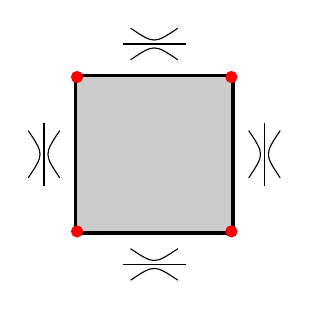
\begin{tikzpicture}[line join = round]
    \node (O) at (0,-0.2) {};
    \draw[] (-0.4,1.4) -- (0.4,1.4);
    \draw[thin] (-0.3, 1.6) .. controls (0,1.4) .. (0.3,1.6);
    \draw[thin] (-0.3, 1.2) .. controls (0,1.4) .. (0.3,1.2);

    \draw[] (1.4,-0.4) -- (1.4,0.4);
    \draw[thin] (1.6, -0.3) .. controls (1.4,0) .. (1.6,0.3);
    \draw[thin] (1.2, -0.3) .. controls (1.4,0) .. (1.2,0.3);

    \draw[fill=black!20!white, draw=black, very thick] (-1,-1) rectangle (1,1);
    \draw[fill, red] (0.98,0.98) circle (2pt) (-0.98,0.98) circle (2pt) (0.98,-0.98) circle (2pt) (-0.98,-0.98) circle (2pt) ;

    \draw[] (-1.4,-0.4) -- (-1.4,0.4);
    \draw[thin] (-1.6, -0.3) .. controls (-1.4,0) .. (-1.6,0.3);
    \draw[thin] (-1.2, -0.3) .. controls (-1.4,0) .. (-1.2,0.3);

    \draw[] (-0.4,-1.4) -- (0.4,-1.4);
    \draw[thin] (-0.3, -1.6) .. controls (0,-1.4) .. (0.3,-1.6);
    \draw[thin] (-0.3, -1.2) .. controls (0,-1.4) .. (0.3,-1.2);

\end{tikzpicture}
\end{document}